\documentclass{beamer}
\usepackage[english,russian]{babel}
\usepackage[utf8]{inputenc}
\usepackage{amsmath}
\usetheme{Warsaw}
\usepackage{listings}
\usepackage{xcolor}
\usepackage{tikz}
\usetikzlibrary{graphs}

\lstset{
    frame=tb,
    tabsize=4,
    showstringspaces=false,
    numbers=left,
    commentstyle=\color{green},
    keywordstyle=\color{blue},
    stringstyle=\color{red},
    emph={baz},
    emphstyle=\textbf
}

\begin{document}

\title{Задачи разрешимости логических формул и приложения\newline Лекция 1. Введение}
\author{Роман Холин}
\institute{Московский государственный университет}
\date{Москва, 2021}

\begin{frame}
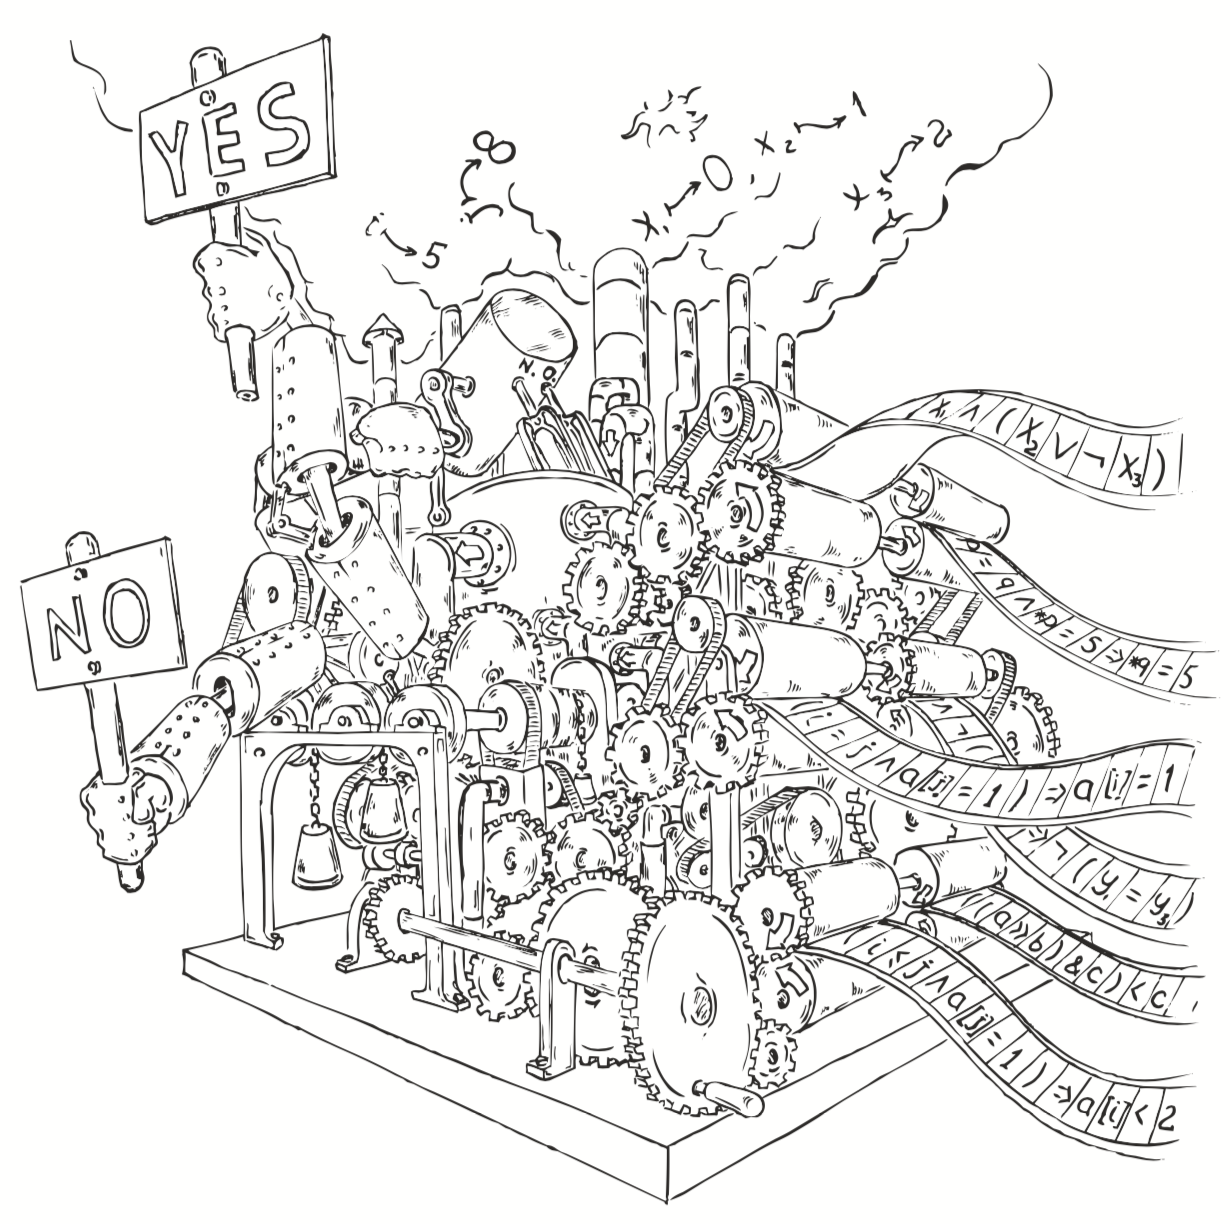
\includegraphics[scale=0.5]{../decision-procedure.png}
\end{frame}

\frame{\titlepage}

\begin{frame}{О чём курс}
\begin{itemize}
\item Что такое решатели
\item Что такое SAT и SMT решатели и чем они отличаются
\item Как ими пользоваться
\item Как они устроены
\item Где они используются
\end{itemize}
\end{frame}

\begin{frame}{Где применяется?}
\begin{itemize}
\item Формальная верификация
\item Поиск ошибок
\item Безопасность
\item Биоинформатика
\item Планирование расписаний
\item Автоматическое доказательство теорем
\item Генерация эксплоитов
\end{itemize}
\end{frame}

\begin{frame}
Edmund Clarke: "a key technology of the 21st century"\newline
Donald Knuth: "evidently a killer app, because it is key to the solution of so mane other problems"\newline
\end{frame}

\begin{frame}{Определения}
Пусть дано множество переменных $V$, скобки и логические связки $\vee$, $\wedge$, $\rightarrow$, $\lnot$. Определим булеву
формулу по индукции:
\begin{itemize}
\item все переменные из $V$ - формулы.
\item если $A$ - формула, то $\lnot(A)$ - формула
\item если $A$, $B$ - формулы, то $(A)\vee(B)$, $(A)\wedge(B)$, $(A)\rightarrow(B)$ - также формулы.
\end{itemize}
\end{frame}

\begin{frame}{Определения}
\begin{itemize}
\item Если $v \in V$, то $v$ и $\lnot v$ называют литералами.
\item Оценка формулы - присвоение каждой переменной значения "истина" или "ложь" и последующее вычисление значения формулы. Значение
формулы вычисляется по индукции.
\end{itemize}
\end{frame}

\begin{frame}{Определения}
\begin{itemize}
\item Булева формула выполнима - если существует такая оценка, что значение формулы при ней "истина".
\item Формула противоречива, если не
существует такой оценки.
\item Формула является тавтологией, если при любой оценки она "истина".
\end{itemize}
\end{frame}

\begin{frame}{Определения}
\begin{itemize}
\item Конъюктивная нормальная форма - форма записи булевой формулы, при которой эта формула имеет вид конъюкции дизъюнкций
литералов.
\item Дизъюнктивная нормальная форма - наоборот.
\end{itemize}
\end{frame}

\begin{frame}{SAT задача}
\begin{itemize}
\item На вход подается булева формула, содержащую только нумерованные переменные, $\vee$, $\wedge$, $\lnot$. Является ли формула выполнимой?
\end{itemize}
\end{frame}

\begin{frame}{SAT задача}
\begin{itemize}
\item Если дизъюнкты в формуле имеет длину не более 2, то сложность задачи распознавания принадлежит классу $P$.
\item Иначе, это $NP$-полная задача (теорема Кука-Левина). Более того, исторически, это первая задача, чья $NP$-полнота была доказана.
\item Что для нас значит, что задача $NP$-полна? Это значит, что если мы каким-то образом научимся решать такую задачу "быстро", то
мы сможем "быстро" решать класс $NP$ задач.
\end{itemize}
\end{frame}

\begin{frame}{Примеры}
\begin{itemize}
\item Вы глава протокола на ужине для иностранных послов в некотором королевстве. Принц хочет, чтобы либо был посол из Перу,
либо не было посла Катара. Королева хочет видить послов Катара или Румынии. Король не хочет видеть послов из Румынии или Перу.
Кого же позвать на ужин?
\end{itemize}
\end{frame}

\begin{frame}{Примеры}
\begin{itemize}
\item Вы глава протокола на ужине для иностранных послов в некотором королевстве. Принц хочет, чтобы либо был посол из Перу,
либо не было посла Катара. Королева хочет видить послов Катара или Румынии. Король не хочет видеть послов из Румынии или Перу.
Кого же позвать на ужин?
\item $(\lnot p \vee q) \wedge (q \vee r) \wedge (\lnot r \vee \lnot q)$
\end{itemize}
\end{frame}

\begin{frame}{Примеры}
\begin{itemize}
\item Пусть множество натуральных чисел разбили на конечное количество непересекающихся множеств. Есть ли хотя бы одно
множество, которое содержит тройку чисел, которая является Пифагоровой? Например, пусть натуральные числа разбили на два
множества: множество четных и множество нечетных чисел. Тогда очевидно, что множество нечетных чисел не содержит Пифагоровой
тройки.
\end{itemize}
\end{frame}

\begin{frame}{Примеры}
\begin{itemize}
\item Давайте упростим задачу: давайте будем делить множество натуральных чисел только на две части. Тогда ответ на задачу
положительный. Достаточно представить подмножество натуральных чисел, которое нельзя разбить на 2 части так, чтобы не в одном
из них не было пифагоровой тройки. С помощью SAT решателя можно выяснить, что наименьшее такое $N$, что множество
$\{1, \dots, N\}$ нельзя разбить на 2 множества, равно $7825$.
\end{itemize}
\end{frame}

\begin{frame}{Примеры}
\begin{itemize}
\item А что, если мы разбиваем на три множества? Можно показать, что множество $\{1, \dots, 10^7\}$ можно разбить.
\end{itemize}
\end{frame}

\begin{frame}{Пример}
\begin{itemize}
\item Зачем разобрали этот пример? Потому что решение этой задачи сродни тому, как мы решаем задачи верификации и поиска ошибок.
После публикации "Symbolic Model Checking without BDDs" 1999 рост интереса людей, занимающиеся верификацией и поском ошибок к
решателям сильно возрос.
\item Поиск ошибок - это поиск контрпримера.
\item Верификация - доказательство того, что контрпримера нет.
\item Сейчас верификаторы и сканеры ошибок - основные "потребители" SAT и SMT решателей.
\end{itemize}
\end{frame}

\begin{frame}{Проверка кода на эквивалентность}
if(!a \&\& !b) h();\newline
else if(!a) g();\newline
else f();\newline
\newline
if(a) f();\newline
else if(b) g();\newline
else h();
\end{frame}

\begin{frame}{Проверка кода на эквивалентность}
Представим процедуры как будевские переменные:\newline
if $\lnot a \wedge \lnot b$ then h\newline
else if $\lnot a$ then g\newline
else $f$\newline
\newline
if $a$ then f\newline
else if $b$ then g\newline
else h
\end{frame}

\begin{frame}{Проверка кода на эквивалентность}
Представим процедуры как будевские переменные:\newline
if $\lnot a \wedge \lnot b$ then h\newline
else if $\lnot a$ then g\newline
else $f$\newline
\newline
if $a$ then f\newline
else if $b$ then g\newline
else h\newline
Скомпилируем код в КНФ:\newline
compile(if x then y else z ) $\equiv (\lnot x \vee y) \wedge (x \vee z)$
\end{frame}

\begin{frame}{Проверка кода на эквивалентность}
Скомпилируем код в КНФ:\newline
compile(if x then y else z ) $\equiv (\lnot x \vee y) \wedge (x \vee z)$\newline
if $\lnot a \wedge \lnot b$ then h else if $\lnot a$ then g else f $\equiv$\newline
$(\lnot(\lnot a \wedge \lnot b) \vee h) \wedge ((\lnot a \wedge \lnot b) \vee ($if $\lnot a$ then g else f )) $\equiv$\newline
$(a \vee b \vee h) \wedge ((\lnot a \wedge \lnot b) \vee ((a \vee g ) \wedge (\lnot a \vee f ))$
\end{frame}

\begin{frame}{Проверка кода на эквивалентность}
Скомпилируем код в КНФ:\newline
compile(if x then y else z ) $\equiv (\lnot x \vee y) \wedge (x \vee z)$\newline
if $\lnot a \wedge \lnot b$ then h else if $\lnot a$ then g else f $\equiv$\newline
$(\lnot(\lnot a \wedge \lnot b) \vee h) \wedge ((\lnot a \wedge \lnot b) \vee ($if $\lnot a$ then g else f )) $\equiv$\newline
$(a \vee b \vee h) \wedge ((\lnot a \wedge \lnot b) \vee ((a \vee g ) \wedge (\lnot a \vee f ))$
\newline
if a then f else if b then g else h $\equiv$\newline
$(\lnot a \vee f) \wedge (a \vee$(if b then g else h)) $\equiv$\newline
$(\lnot a \vee f) \wedge (a \vee((\lnot b \vee g) \wedge (b \vee h))$
\end{frame}

\begin{frame}{SMT решатель}
\begin{itemize}
\item Что, если нам хочется задавать более сложные вопросы решателю? Например, разрешима ли такая формула:
$(x = 4) \wedge ((y = 7) \vee (x = y))$
\item Или такая: $(x + y = 3) \wedge (y - z = 7) \wedge (z * 2 = 4)$
\item Или такая: $(lenght(s) = 3) \wedge (s[0] = 'a') \wedge (s[1] = 'b') \wedge (s[2] = 'c')$
\end{itemize}
\end{frame}

\begin{frame}{SMT решатель}
Пропозиционной логики для этого не достаточно. Для описания таких систем используется логика первого порядки и теории.
\begin{itemize}
\item равенства
\item равенства и неинтерпритируемых функций
\item линейной арифметики
\item векторы битов
\item массивов
\end{itemize}
Большая часть SMT решателей использует SAT решатели.
\end{frame}

\begin{frame}{SMT-lib}
\begin{itemize}
\item Специальный list-подобный язык для записи уравнений, подающийся на вход решателю.
\end{itemize}
\end{frame}

\begin{frame}{SMT-lib}
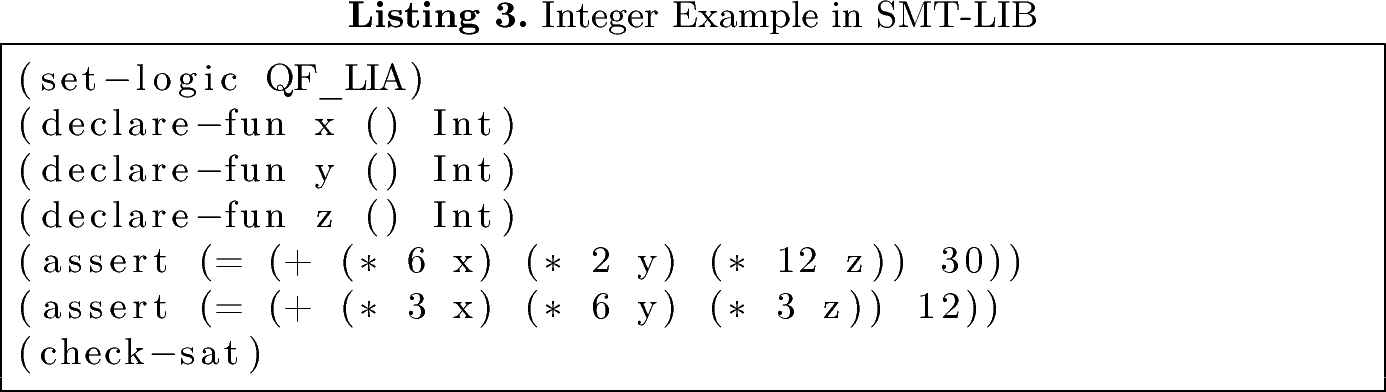
\includegraphics[scale=1.0]{SMT-LIB.png}
\end{frame}

\begin{frame}{}
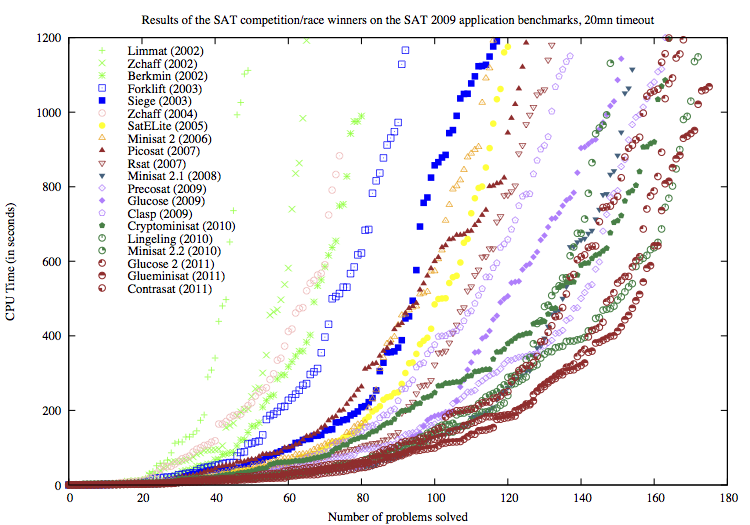
\includegraphics[scale=0.4]{SAT_results.png}
\end{frame}

\begin{frame}
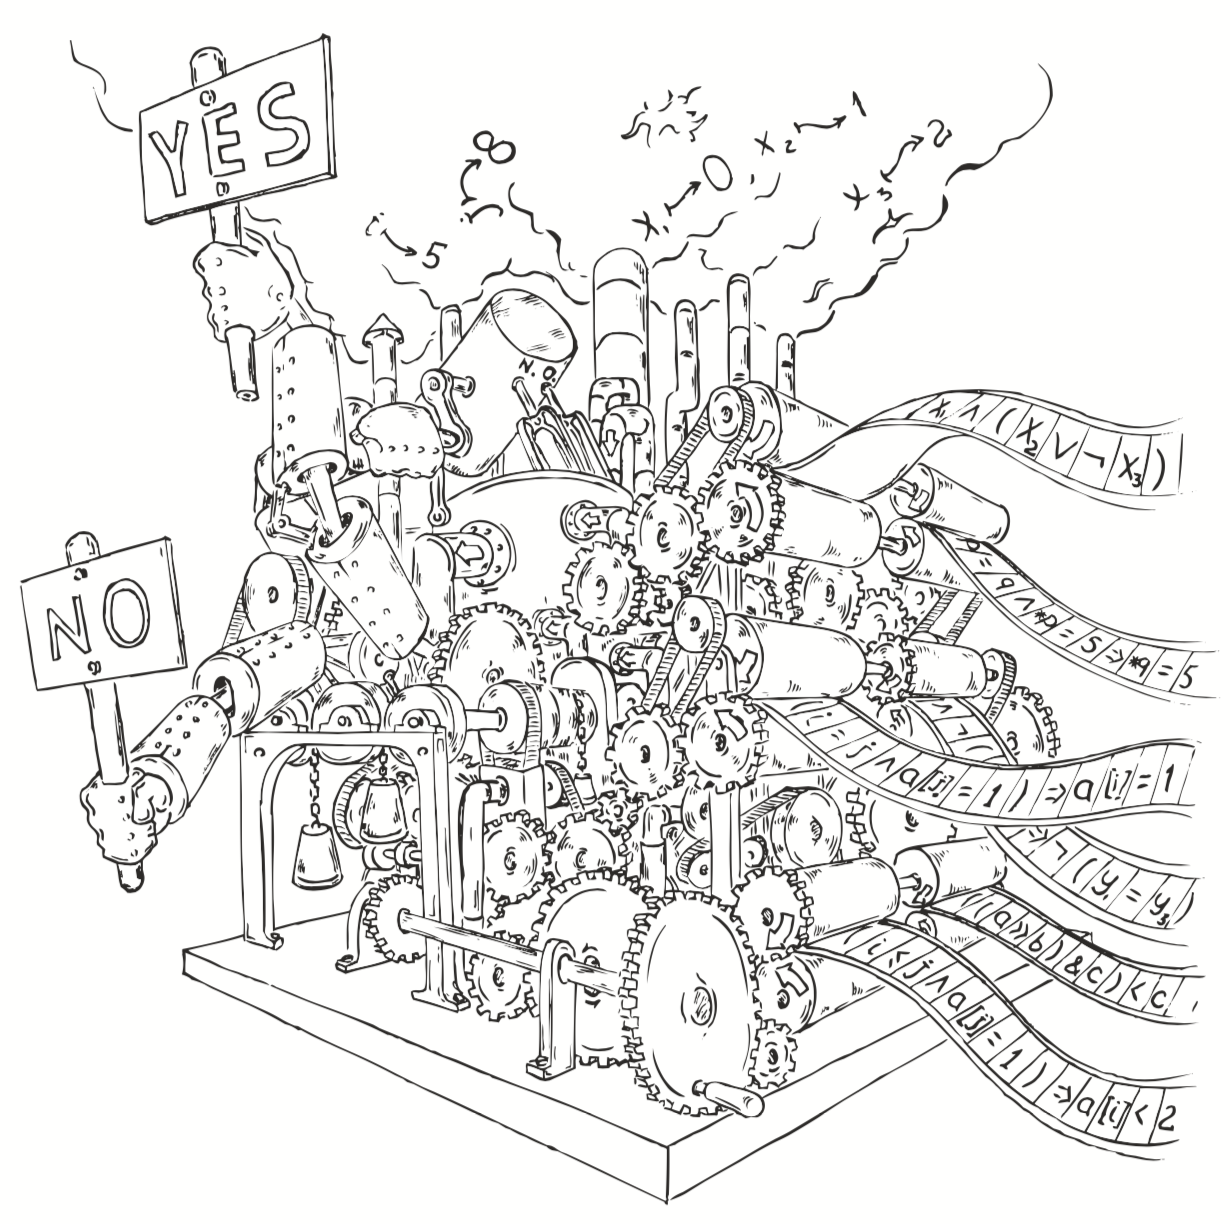
\includegraphics[scale=0.5]{../decision-procedure.png}
\end{frame}

\end{document}
